\chapter{Introduction}
% 20 pages or so
% rules of the game
% objective of my algorithms
% literature review

\section{Robotic Coverage Background}

Robotic motion planning problems are typically concerned with finding an achievable path between two robot configurations. These configurations could be the current location of a robotic vehicle along with its desired destination, the current pose of a robotic arm and the pose required for it to grasp an object, or any other pair of robot states that correspond to ``start" and ``goal" configurations. \textit{Robotic coverage} problems are another kind of motion planning problem. The goal of a robotic coverage problem is to find a path for the robot to follow during which it will visit every location in a region. This region could be an area of floor to be vacuumed, the surface of a car body that needs to be painted, or the interior of a building that needs to be mapped. In all of these cases, the task is only complete once the entire region has been visited, or \textit{covered} by a robot. Usually, another goal of these problems is to achieve coverage in a way that minimizes the time or number of movements required to complete the task. The robotic coverage problem can be viewed as a continuous generalization of the traveling salesman problem \cite{Arkin1993}. Thus, the general form of the problem is NP-Hard. Applications for robotic coverage continue to be developed today. For example, work by \citeauthor{Daltorio} from 2010 develops control policies necessary to achieve "obstacle edging" behavior \cite{Daltorio}. This work effectively implements ideas from algorithms that perform online coverage of an unknown environment, discussed shortly.

% based on Choset, section 1. Is this too similar to the original?
%should I elaborate on the early heuristic algorithms that did not guarantee coverage
One particularly well studied type of robotic coverage problem is the case where the coverage region is some subset of the plane, and the robots are mobile robots that can only move in the plane. A good overview of this kind of coverage problem can be found in \cite{Choset}. Algorithms to perform robot coverage in the plane have been studied since the late 1980's. Early algorithms for this purpose relied on the use of heuristics, and these algorithms usually could not guarantee that complete coverage would be achieved for all possible environments. By around 2000, several planar coverage algorithms were able to guarantee complete coverage for a variety of simple environment types. Many of these algorithms proved completeness by showing that the algorithm breaks down the coverage space into smaller regions that are relatively trivial to cover completely. Coverage algorithms that employ this kind of technique are known as \textit{cellular decomposition} algorithms.

One type of cellular decomposition fits a square grid to the coverage space. Because a general arbitrary set in the plane can not be exactly expressed as a union of grid-aligned square regions, this technique is often called approximate cellular decomposition. Typically, each cell in this kind of decomposition can be covered entirely by a single robot configuration. For example, consider dividing a grass lawn into squares for a robotic lawn mowing task. If each square in the cellular decomposition is small enough, a lawnmower whose center is aligned with a square's center will have mowed that entire square of the lawn. In coverage problems where this assumption applies, proving that a coverage path visits each cell in the approximate decomposition is sufficient to guarantee complete coverage.

In addition to approximate cellular decomposition, there are also techniques that decompose a coverage space into a more diverse collection of cell shapes. Examples of such shapes include cells of fixed width whose top and bottom boundaries can vary in shape \cite{Hert1996}, or trapezoidal cells whose parallel sides all run in the same direction \cite{Choset-2000}. Depending on whether the union of these cells is exactly equal to the coverage space, such techniques are called either \textit{semi-approximate} or \textit{exact} cell compositions. In the case of trapezoidal cell decomposition, it is possible to combine the trapezoidal cells into a smaller number of large cells, each of which are able to be covered by a simple back-and-forth sweeping motion. This approach is known as a \textit{boustrophedon} decomposition \cite{Choset-2000}.

\begin{figure}[H]
%\centering
\begin{subfigure}{.5\textwidth}
  \centering
  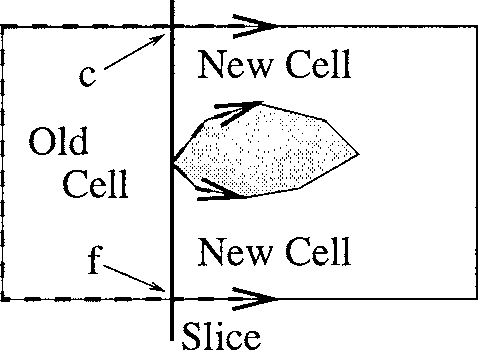
\includegraphics[width=.5\linewidth]{boustrophedonSplit}
  \caption{Two new cells created at critical point}
\end{subfigure}
\begin{subfigure}{.5\textwidth}
  \centering
  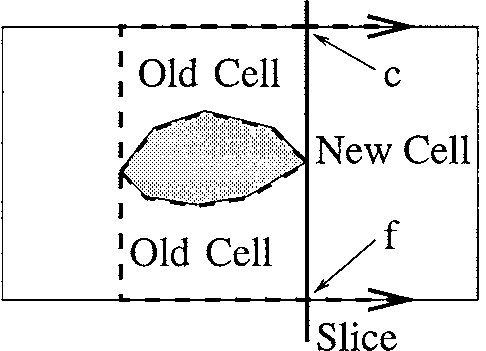
\includegraphics[width=.5\linewidth]{boustrophedonCombine}
  \caption{Transition from two cells to one new one}
\end{subfigure}
\caption[Boustrophedon Decomposition]{Boustrophedon cell creation at critical points}
\end{figure}

\subsection{Spanning-Tree based Coverage Algorithms}

When coverage is performed by a square shaped tool attached to a mobile robot, and when the coverage area can be exactly decomposed into a grid of squares that have double the side length of the robot tool, it is possible to compute an optimal covering path in linear time using an approach based on spanning trees \cite{STC}. Gabriely and Rimon developed several variants of this approach with different time, memory, and prior knowledge requirements. In all cases, it was assumed that a mobile robot would complete the coverage task with a square shaped tool of size \textit{D}. It was also assumed that the tool could only move in the four cardinal directions when completing the task. Finally, it was assumed that the region to be covered could be approximated by cells in a grid of squares with size 2\textit{D}. The authors argue that the final assumption is justified for realistic environments in which the size of the robot's tool is significantly smaller than the dimensions of the area to be covered. Under these assumptions, the \textit{Spanning Tree Covering} (STC) algorithm is able to generate a path through the space which visits each grid-aligned square cell of size D exactly once.

\begin{figure}[H]
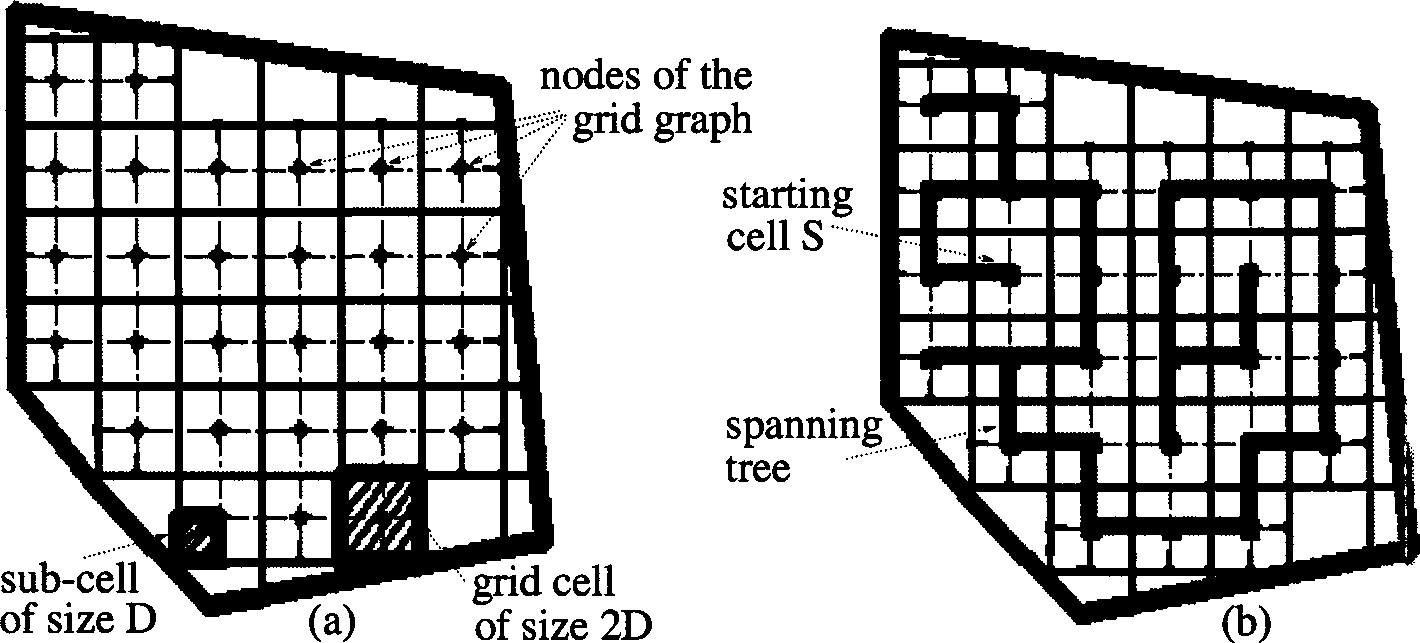
\includegraphics[width=\textwidth]{gridAndSpanningTree}
\caption[Spanning Tree Example]{A small coverage environment and a spanning tree on that environment \cite{STC}.}
\end{figure}

The offline variant of STC works by representing the coverage area as a graph \textit{G}. Nodes on this graph represent the center of a square with size 2\textit{D}, and the set of nodes corresponds to the set of full cells when a grid with square size 2\textit{D} is overlaid on the coverage space. Edges exist between any two nodes whose corresponding cells are adjacent in the coverage space. As the name suggests, STC's key step is the creation of a spanning tree on \textit{G}, using any node in \textit{G} as the root of the tree. Many algorithms exist to compute spanning trees, but two popular examples are based on breadth-first-search and depth-first-search \cite{CormenAlg}.

Once this spanning tree has been created, the coverage area is subdivided into squares of size \textit{D}. Each node of \textit{G} coincides with the corners of four different squares in this subdivided map. Starting at any one of these squares, each of which is exactly the shape and size of the robot's coverage tool, the robot can simply move counterclockwise around the spanning tree as if it were performing wall following. In this way, each cell in the coverage space will be visited exactly once by the robot. Because of this property along with the fact that the path generated by STC ends in a position adjacent to where it started, the path found by STC can be considered a Hamiltonian cycle on \textit{G}. Although constructing a Hamiltonian path on a general planar grid is NP-complete \cite{Itai}, the assumed properties of \textit{G} make it practical to compute such a path on this graph in linear time. The fact that this coverage path's start and end positions will be in adjacent cells can be beneficial in practice, as it allows deployment and retrieval of the robot to happen in approximately the same place.

\begin{figure}[H]
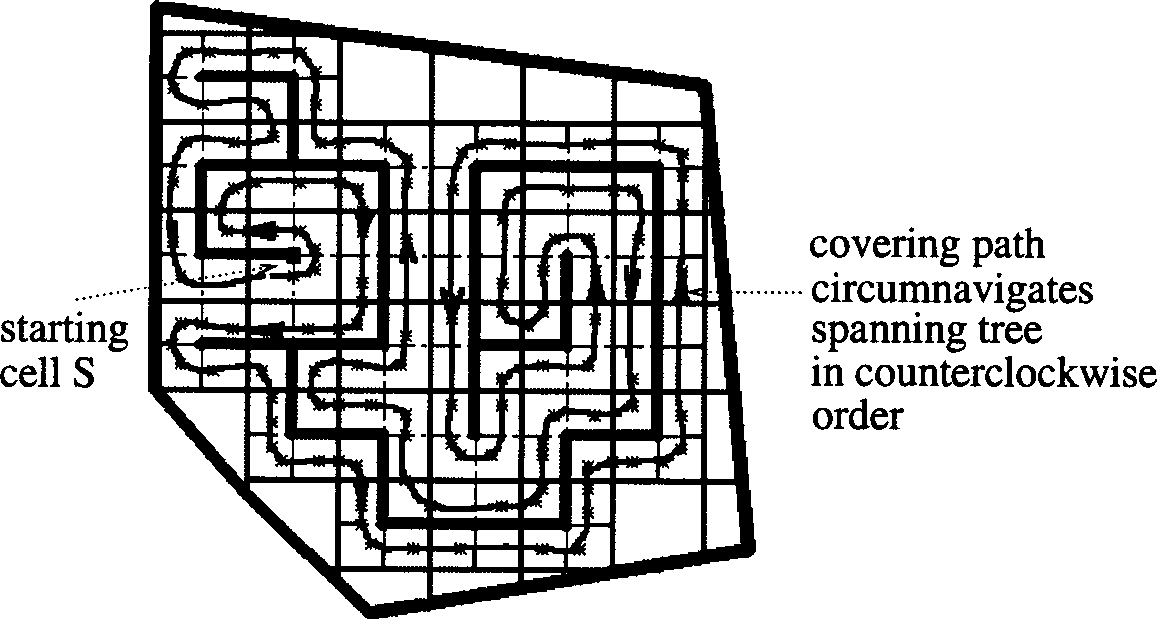
\includegraphics[width=\textwidth]{spanningTreeWithPath}
\caption[Spanning Tree Coverage Path]{Following the spanning tree of \textit{G} achieves exact coverage and creates a cycle \cite{STC}.}
\end{figure}

This algorithm has a few interesting variants. The first runs online, and effectively circumnavigates a depth first search spanning tree that it constructs on the fly \cite{STC}. Restriction to use of depth first search is the primary disadvantage of this approach compared to offline STC. While the coverage paths based on depth first search are equivalent to those created through any other method in terms of final path length, other spanning tree algorithms have practical benefits. For example, spanning tree algorithms such as Prim's algorithm or Kruskal's algorithm can create minimal spanning trees on weighted graphs. For details on Prim's algorithm and Kruskal's algorithm, refer to \cite{CormenAlg}. Setting the weights in a particular way can lead to coverage paths with desirable properties. For example, a minimal spanning tree on a graph where North-South edges are given less weight that East-West edges will tend to move in long, parallel lines that minimize turning. In later work, Gabriely and Rimon develop an online approach called Scan-STC that achieves similar behavior. Scan-STC also makes additional improvements on the original STC as discussed below.

The second online variant of the STC algorithm is described by Gabriely and Rimon as \textit{ant-like}. In this case, the robot must be able to mark visited sub-cells through some means such as leaving pebbles on the ground. In addition, the robot must be able to sense the presence of these makers in the nodes of \textit{G} adjacent to its current position. By marking each visited sub cell as the robot leaves that cell, the robot is able to proceed on the same path it would have created in the depth first search based online approach. Because this algorithm uses markers to identify visited nodes, it requires only O(1) memory. However, it requires the use of O(N) markers, where N is the number of sub-cells in the coverage area. Nonetheless, this algorithm presents interesting ideas for multi-agent approaches and prevention of drift in pose estimation. In both of these cases, physical and immobile records of a robot's past location can inform the decision making of any robot currently near some of those records.

\begin{figure}[H]
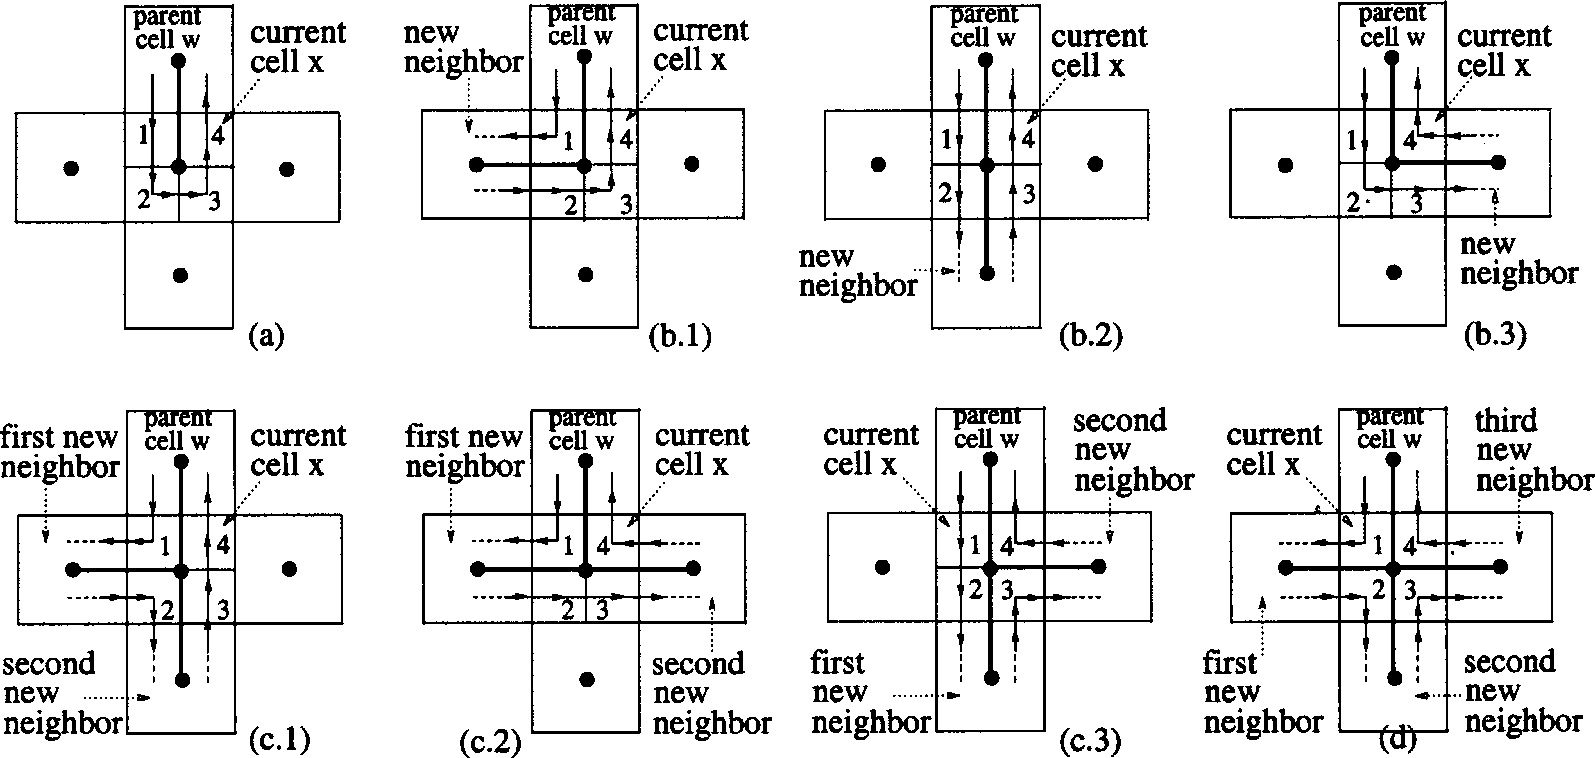
\includegraphics[width=\textwidth]{motionPermutations}
\caption[Neighbor Visiting Behavior for Online STC]{Online STC variants determine their behavior according to current position and whether neighbors have been visited before \cite{STC}.}
\end{figure}

Finally, there is a variant of STC that achieves \textit{exact} coverage of an environment, even when that environment can not be represented by completely filled cells on a grid of squares with size 2\textit{D}. However, this approach still requires that the connectivity of the environment is represented adequately by such a grid. The resulting algorithm simply notices any cells that are partially occupied by a previously unseen obstacle when it passes next to them in the course of normal online STC. When such a cell is encountered, a neighborhood is swept around the entire obstacle. Then, the robot returns to traversing the fully in-bounds cells according to its usual procedure. The ability to complete this sweeping motion is always guaranteed under assumptions used to model this problem. For details concerning the size of this neighborhood and the correctness of the resulting algorithm, see \cite{STC}.

In the previously mentioned Scan-STC algorithm, Gabriely and Rimon improve STC to explicitly handle boundary cells, or graph cells that are partially occupied by an obstacle. Using the same notation as before, this algorithm generates a path with length no greater than $ (n + m)\textit{D} $, where n is the number of nodes in \textit{G}, and m is the number of boundary cells \cite{Gabriely2003}. The authors assume that no node will contain an arrangement of obstacles such that the graph of that node's sub-nodes is disconnected. If an obstacle exists such that the normal grid of nodes would violate this assumption, the corresponding location in the coverage area is assigned two different nodes. With that assumption in place, avoidance of obstacles is done by simply displacing the normal path that goes around the obstacle. This displacement tactic is what leads to the m term appearing in the maximum path length bound. The authors claim that in practical environments, the path length is closer to $ n + \frac{m}{2} $. 

\begin{figure}[H]
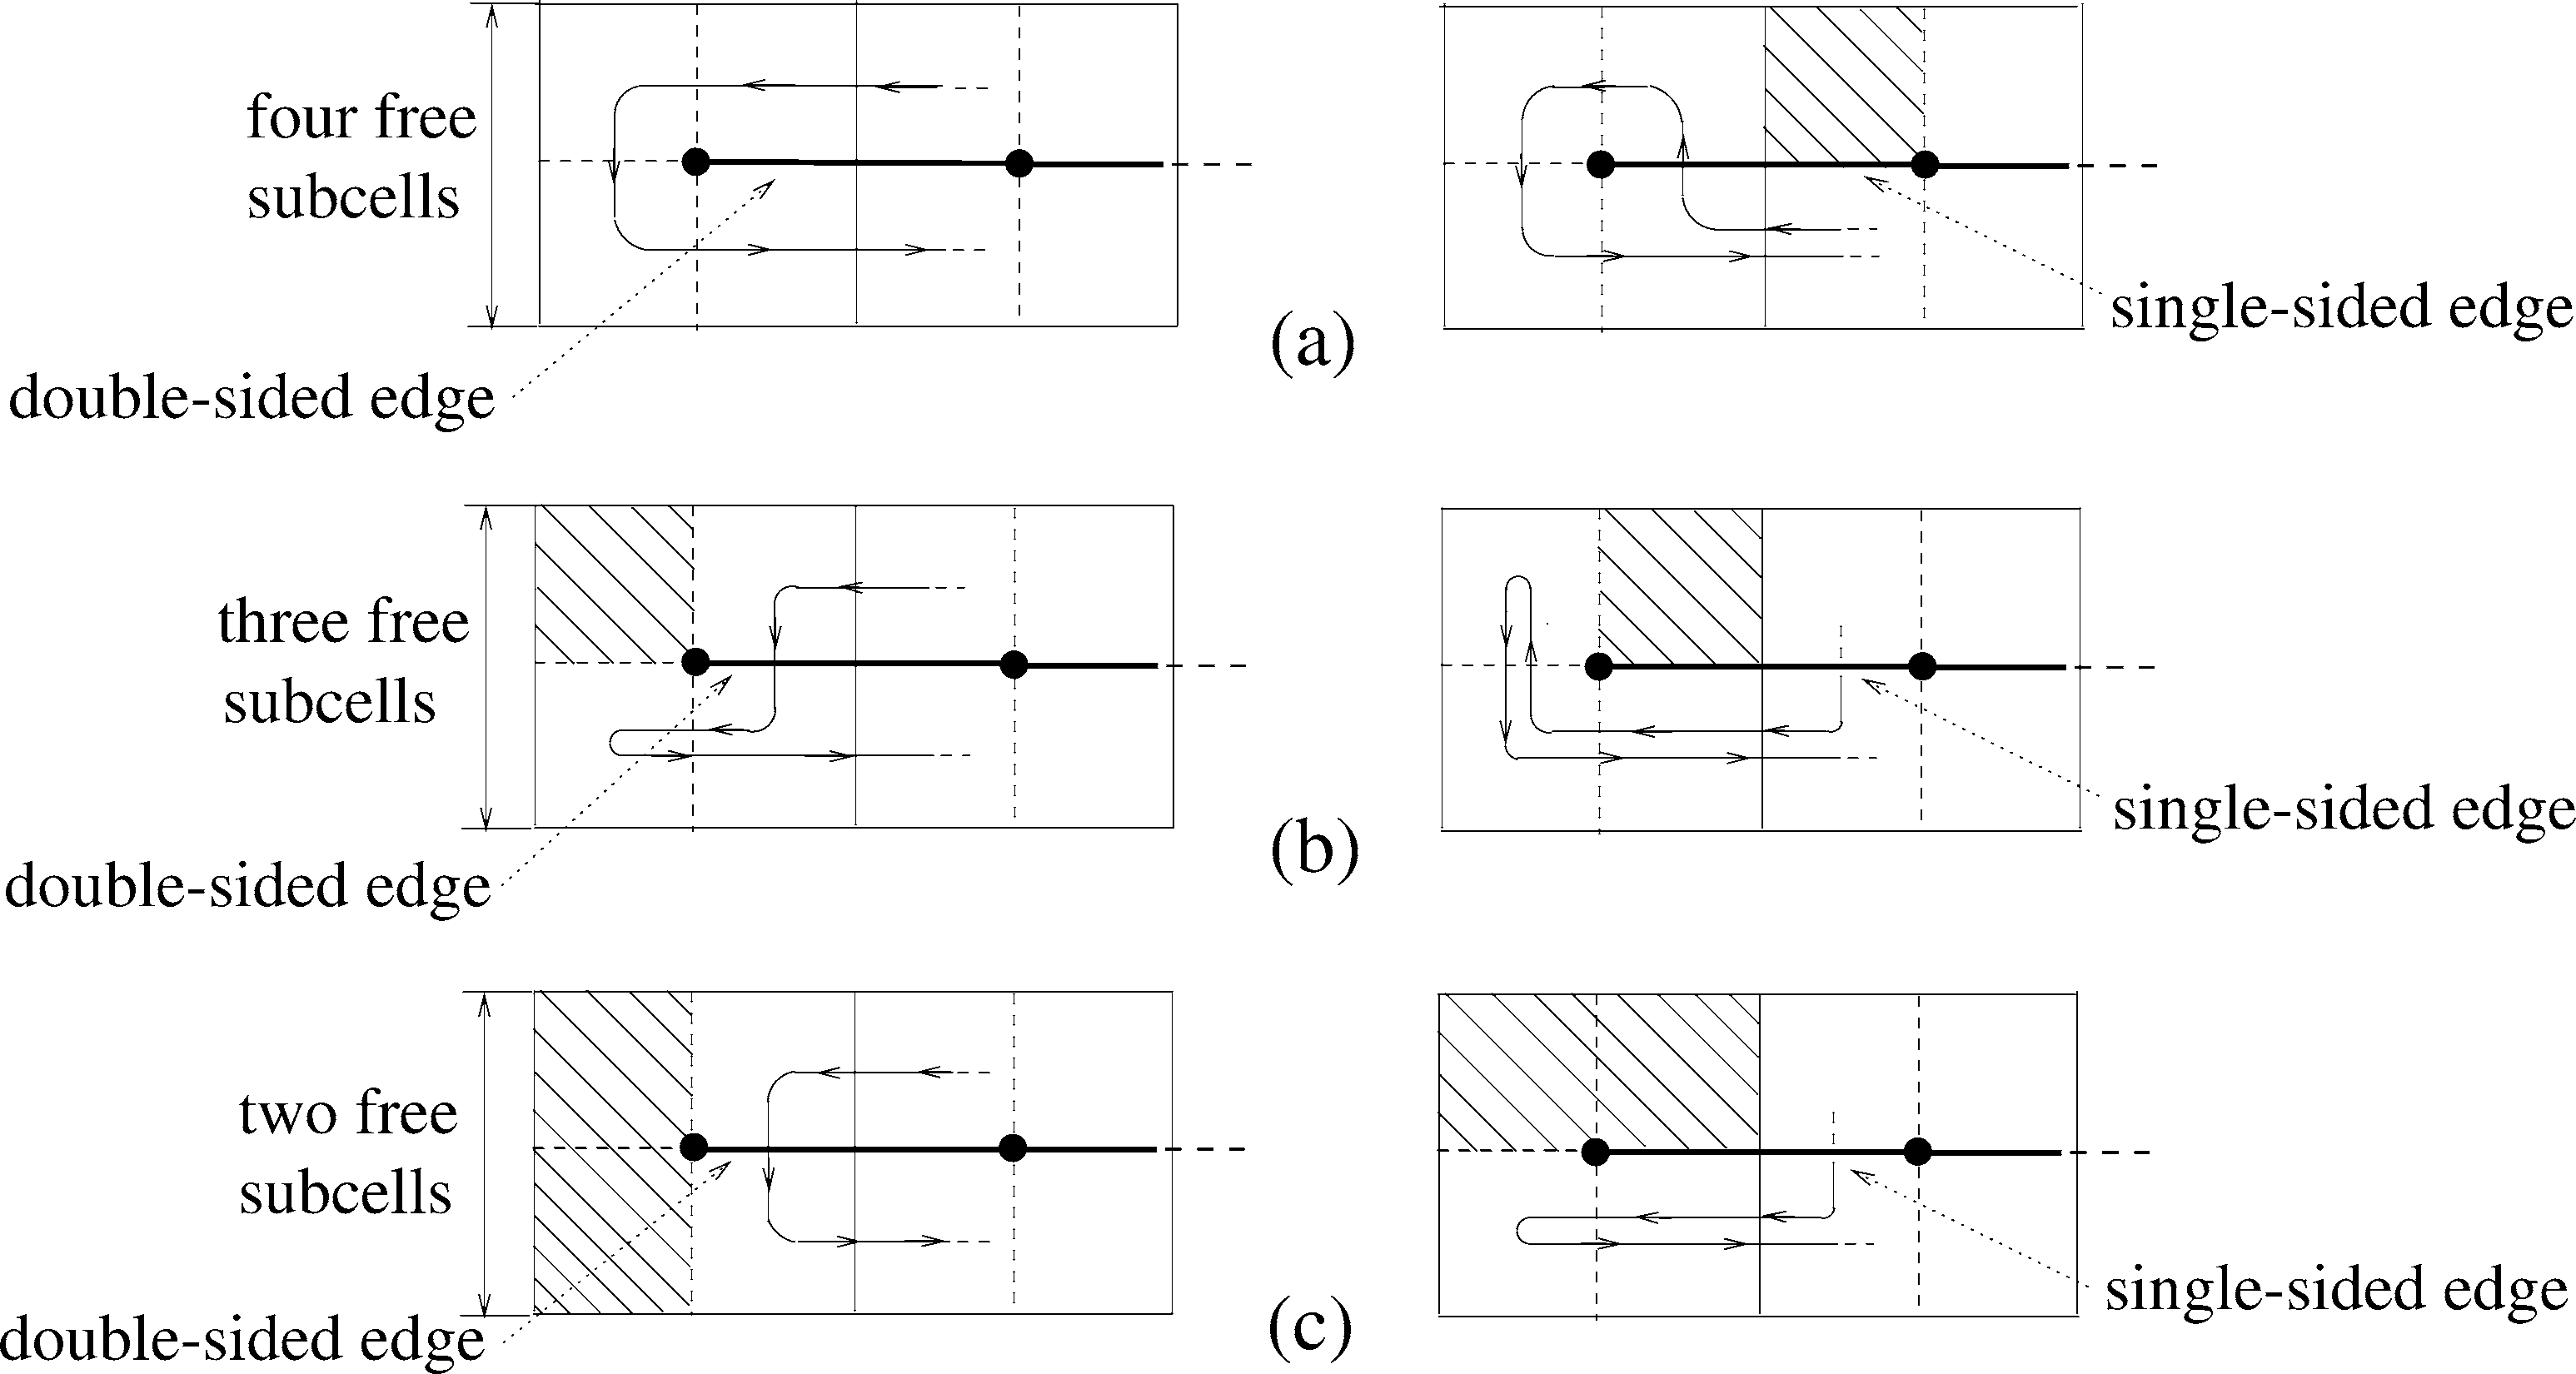
\includegraphics[width=\textwidth]{pathDeformationsScanSTC}
\caption[Path Deformations in Scan-STC]{Scan-STC adapts its motion in a variety of situations with partially occupied cells \cite{Gabriely2003}.}
\end{figure}

%%illustrate an example of a node whose subnodes are disconnected (2 out of bounds non-adjacent subcells)

The other significant insight of Scan-STC relates to its name. By allowing the mobile robot to sense the state of the eight cells the surround its current position, it is possible to discover that one of the horizontal neighbors of the current cell has a free vertical neighbor, and that the current cell has a free vertical neighbor in the same direction. In this case, it is guaranteed that a path into the node's horizontal neighbor exists such that the vertical neighbors of these cells appear between the current cell and its horizontal neighbor. With this insight, it is possible to skip the creation of a horizontal edge between the current node and its horizontal neighbor. The benefit of this approach is that it leads to coverage paths that move primarily in the vertical directions. This can be useful for limiting the amount of turns performed, thereby reducing the number of opportunities to introduce dead reckoning error from imprecise turns.

\subsection{Multi-Agent Robotic Coverage}

Another imprint feature of a robotic coverage algorithm is whether that algorithm controls a single robot or a group. Multi-agent robotic coverage algorithms address the latter case. Multi agent approaches to coverage can often complete a coverage task several times faster than a single agent approach because of the division of work that use of multiple robots enables. Use of multiple robots can also enhance robotic coverage by allowing for more precise localization through information sharing. Finally, multi-agent methods are often able to adapt to the failure of one or more robots, as there may be remaining robots capable of completing the coverage task \cite{Choset}. As robotic hardware decreases in price, taking full advantage of these benefits is increasingly viable in terms of up-front costs. However, multi-agent techniques often require more complex motion planning strategies to coordinate the motion of multiple robots in a way that takes full advantage of these potential efficiency improvements and other benefits.

%probably good to do a more general list of multi agent coverage algorithms before going straight into multi agent STC variants

A large amount of research adapts the spanning tree approach to the case of multi-agent coverage \cite{Zheng}\cite{Hazon}. In their work on this subject, Noam Hazon and Gal Kaminka generalize the STC algorithm to the multi agent case, resulting in an algorithm called \textit{Multirobot Spanning-Tree Coverage}, or MSTC. The MSTC problem assumes that the coverage area can be adequately approximated by a grid of square cells with side length 2\textit{D}, as in the spanning tree coverage algorithm. As with the \textit{original} version of STC, it is assumed that all cells in the coverage space are free of obstacles. It is also assumed that all robots have the same speed and tool size. A version of this assumption, that all robots are the same, applies to most of the work on multi-agent robotic coverage.

%describe notable exceptions to the above where coverage is done with heterogeneous agents

With these assumptions in place, the first version of MSTC simply constructs a spanning tree of the space offline, then has all of the drones start to follow the spanning tree from their initial positions, much the same as single agent STC. If the robots are able to share information about their status, i.e. working or broken, and whether they have completed their assigned section, then it is possible to have all working robots continue to follow the spanning tree path until the coverage task is complete. Under these assumptions, complete coverage is guaranteed as long as one robot remains in working order until the end of the task.

\begin{figure}[H]
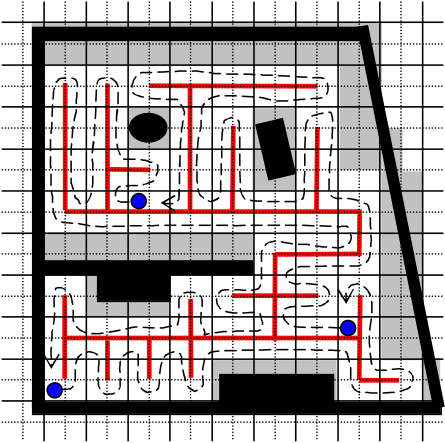
\includegraphics[width=0.5\textwidth]{mstcPathFollowing}
\caption[MSTC Path Following Behavior]{The MSTC algorithm assigns portions of a shared loop to each drone based on its starting position \cite{Hazon}.}
\end{figure}

If there are k robots exploring a coverage space with n sub-cells as described above, then the best case time for this algorithm is shown to be $ \frac{n}{k} - 1 $. This performance is achieved when the starting points of the robots are distributed such that each robot is evenly spaced along the length of the spanning tree coverage path. The worst case is stated to be $ n - k - 1$, for the case where all k robots start on k adjacent sub-cells that appear together in the spanning tree graph. Implicit in both bounds is the assumption that no robots fail. In a pathological case with the same initial conditions used to give the previously stated worst case bound, the $ k - 1$ robots that start directly in front of the last robot could all fail at time $ n - k - 2$, just before the front robot reached the back robot's position. In this case, it would take another $n - 1$  steps for the remaining robot to complete the coverage task according to Algorithm 2 as described by the authors, leading to a total coverage time of $ 2 n - k - 2 $. The authors note that many practical multi-robot coverage scenarios require starting all robots from the same location, meaning that performance close to the worst case bound $ n - k - 1 $ is relatively common. This motivates the development of a more sophisticated coverage algorithm. By assuming that backtracking is allowed, the authors develop an algorithm with a worst case of $ \frac{n}{2} - 1 $ for $ k > 2 $. However, because all algorithms in \cite{Hazon} only consider the possibility of moving forward and backward along the initially calculated spanning tree path, many opportunities for further improvement remain.

Work by Zheng et al. surpasses the average-case performance of MSTC with their \textit{Multi-Robot Forest Coverage} (MFC) algorithm \cite{Zheng}. As the name suggests, MFC computes a separate spanning tree for each of the robots working on the coverage task. For convenience, the authors of MFC also assume that multiple robots can occupy the same sub-cell simultaneously, and that the coverage area can be represented by grid-aligned cells with side length twice that of the robot's coverage tool. Experimental results showed that MFC achieved performance close to a theoretical lower bound in many cases.

\begin{figure}[H]
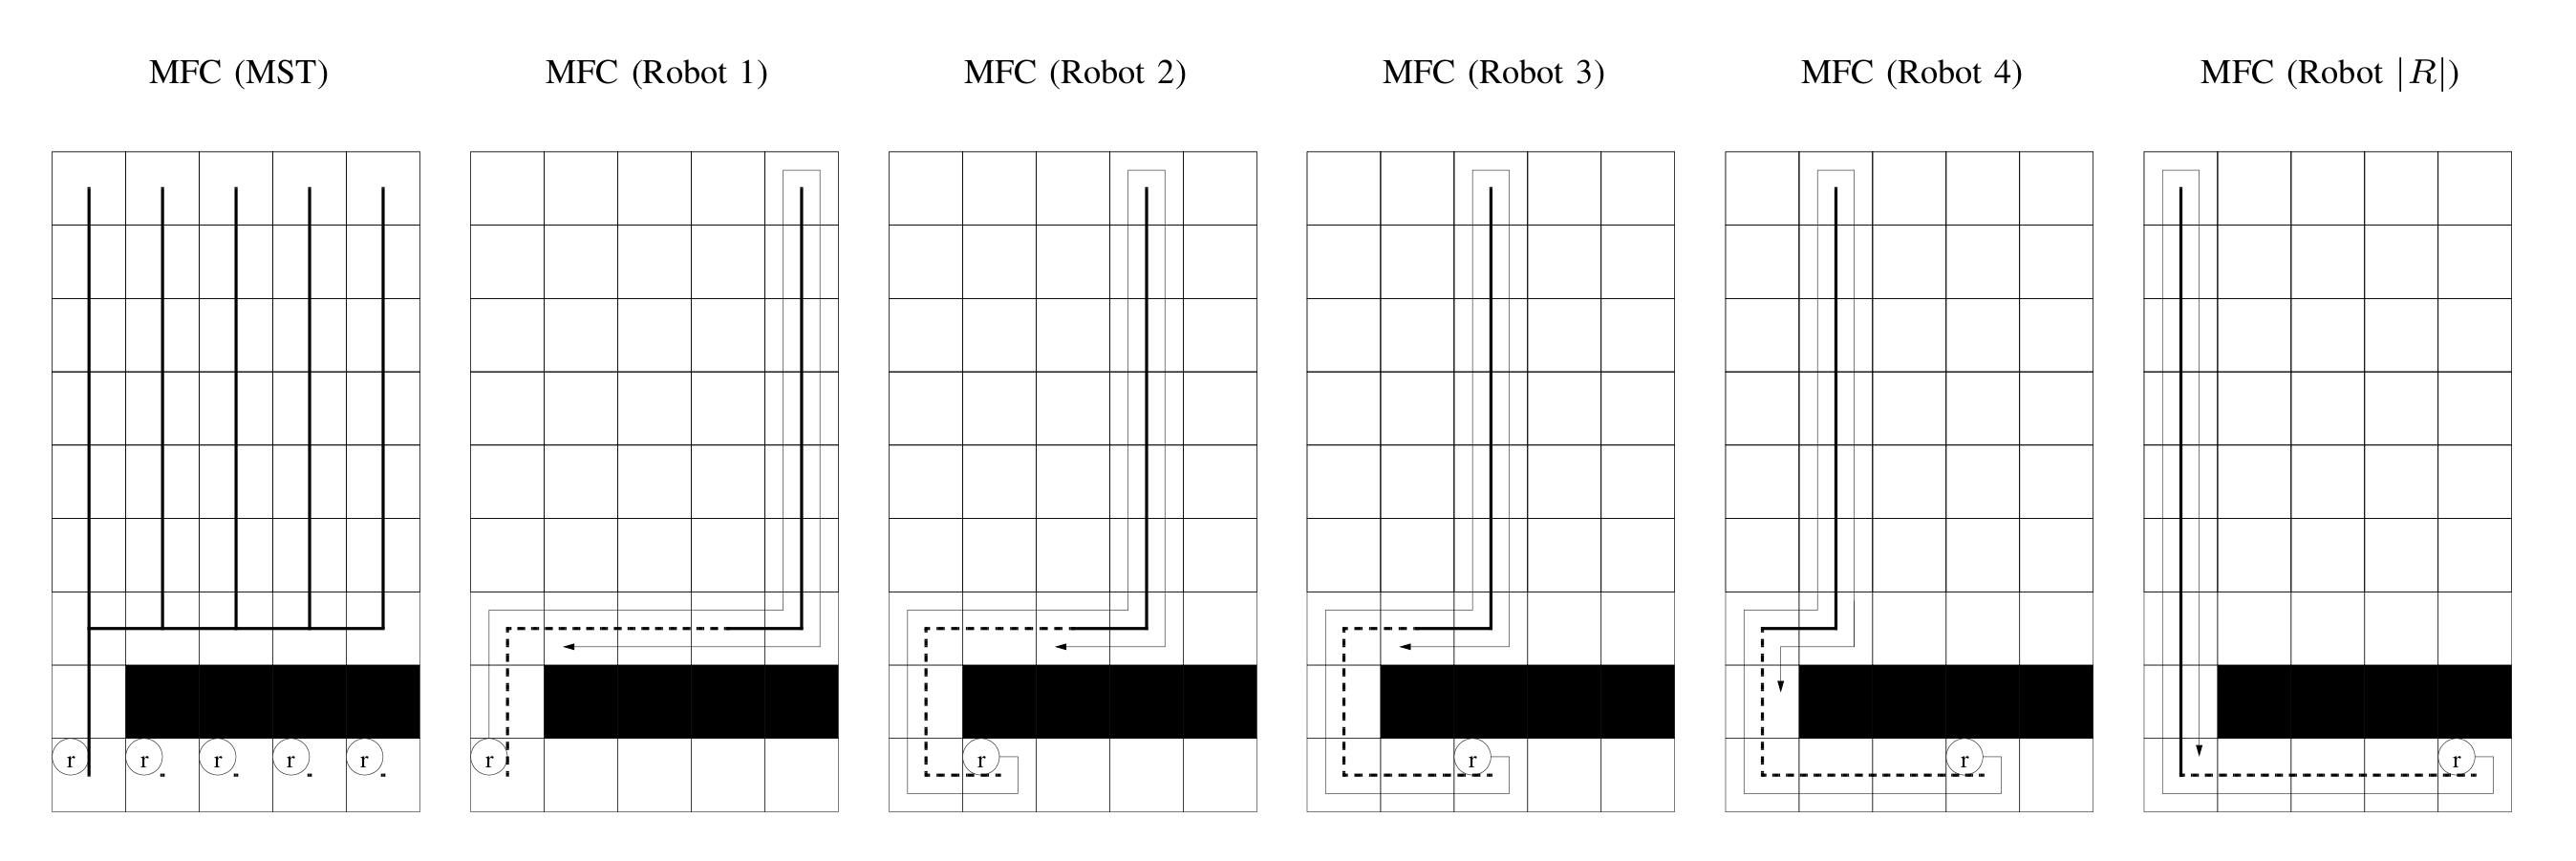
\includegraphics[width=\textwidth]{mfcBreakdown}
\caption[Multi-Robot Forest Coverage Path Creation]{MFC assigns a different spanning tree to each robot.}
\label {fig:MRCPaths}
\end{figure}

In addition, Zheng et al. were able to prove that their algorithm's cover times are no worse than eight times the optimal value, thanks to properties of a tree cover algorithm for general graphs that they adapted to this purpose. The tree cover algorithm, developed by Even et al, finds a forest of $|R|$ trees that start from a set $R$ of root positions and cover an entire graph $G = (V, E)$. This algorithm attempts to minimize the largest weight of its trees. The algorithm runs in polynomial time and finds forests such that the maximum tree weight is no more than four times larger than optimal. Zheng et al. use a lightly altered version of this algorithm to determine the individual trees assigned to each robot in the space (Figure \ref{fig:MRCPaths}). 

\section{Problem Statement}

As with most of the previously discussed research, this work presents multi-agent coverage algorithms based on spanning trees. The details of the coverage problem stated here vary somewhat from other work - these differences are motivated by a use case in which a team of aerial drones (UAVs, robots) must use cameras or other 2D imaging sensors to perform coverage of an area affected by disaster. Practical applications of this work would employ a combination of human effort and image recognition / processing techniques to identify people in need of aid, key structural damage that requires immediate repair, or other points of interest. Once any such point of interest has been identified and located, the relevant information can be used to guide response efforts.

Two particularly novel features are introduced to fit this setting:
%line spacing issue here
\begin{enumerate}
	\item Robots that are able to change the size of their field of view
	\item Environments with subsections that require different levels of scrutiny
\end{enumerate}

These two changes are closely related to one another. Specifically, the varying scrutiny requirements motivates the use of techniques that trade off between an observation's field of view and its level of detail. In turn, concrete motivation for an environment that requires varying levels of scrutiny is based on the idea that not all areas are worth viewing in great detail when gathering information for a search and rescue effort. For example, some areas of the coverage environment may consist of a fairly uniform surface such as a body of water or a large area of flat, rocky terrain. Such areas may not be worth covering in detail because their uniform nature makes it easy to conclude that nothing of interest exists in these regions. At the opposite extreme, trying to observe a region with dense tree cover may not be practical in a coverage scenario constrained by an urgent timeline. In contrast, it may be worth looking closely at areas with partial occlusions, areas with visually complex damaged structures, or places where people are particularly likely to be in need of help.

As with the identification of actual people and other points of interest, the visual identification of which regions are likely to contain useful information that can be practically observed is abstracted away by this work. In its place, this work assumes access to a perfectly accurate sensor that describes the level of scrutiny required to view each environment cell in a drone's field of view. Another assumption of this problem is that the distribution of locations requiring one level of scrutiny or another is not known in advance of coverage. In practice, it may not be possible to know the exact location of collapsed structures, flooded regions, or other environment features that may appear without warning in an emergency.

The other significant novel feature of this problem formulation, robots with a variable field of view, arises naturally as a strategy to adapt to the varying scrutiny requirements of an environment. In this setting, the dimensions of a drone's field of view corresponds to the size of a robot's covering tool in a more traditional presentation of robotic coverage. This work assumes that a drone's field of view is always centered on a point directly below the drone, roughly corresponding to down-facing camera mounted on the bottom of a drone. Real drones can usually alter the size of a ground area being photographed. For example, increasing the size of the observed area may be achieved by ascending with a constant viewing angle or by using an optical camera zoom feature to increase the viewing angle. Likewise, decreasing the field of view may be achieved by descending, zooming in, or by some combination of these.

Increasing the field of view has the obvious benefit of allowing a robot to cover more of its environment at once. Decreasing the field of view increases the detail with which a drone observes the area directly below it, and this allows high detail viewing of those areas for which a highly detailed view has been deemed useful. While the distribution of environment sections that require low vs high scrutiny is unknown a priori, it is assumed that the boundaries of the coverage area and of the obstacles that border it are known in advance.

%go into specifics about the FOV sizes and levels of scrutiny I use here!!!

\subsection{Rules for Robot Motion}

As previously stated, each drone in this formulation has access to moves that increase and decrease its field of view. For simplicity, it is assumed that a drone's field of view can be in only two states that correspond to two possible altitudes. A drone flying low can view a single cell in the environment's approximate cellular decomposition. A drone flying high can view a 3x3 grid of these environment cells. Depending on which altitude the drone currently occupies, it has access one of two vertical motions: ascend and descend. A somewhat arbitrary assumption of this work is that these vertical motions each take about the same length of time as moving cardinally between the centers of adjacent environment cells.

Unlike most other work on spanning-tree based coverage, this work assumes that the robots can move along diagonals, rather than only in the four directions orthogonal to the sides of its tool. For convenience of notation, the four directions commonly used by spanning tree robots will be referred to as \textit{cardinal directions}, and the four directions that are offset by $\frac{1}{8}$ turn from the cardinal directions will be called intercardinal directions. In addition, concrete examples shown in this work may refer to a particular cardinal direction such as East, or a particular intercardinal direction such as South-West (SW).

One reasonable concern about the introduction of diagonal motion in a world represented by an approximate cellular decomposition is how it affects the connectivity of the coverage area. As with many coverage techniques that employ an approximate cellular decomposition of the environment, this work assumes that coverage paths will move directly from the center of one cell (node, patch, location) to the center of one of its neighbors. In addition, it is assumed that the robots are able to move directly between cells that share only a corner, even if one or both of the adjacent cells that would connect them are out of bounds. Since other work typically assumes that the robot is roughly the same size as the area it covers, this assumption requires justification. Because the problem explored here is motivated by a team of autonomous drones observing an area from above, it is safe to assume that the robots are significantly smaller than the area they are actively observing at any particular moment. In addition, the set of in-bounds cells is assumed to represent any cells that are completely covered by terrain to be observed, and so out of bounds cells may correspond to areas that are not \textit{completely} obstructed. Finally, due to the ability of aerial drones to move in three dimensions, it is often possible for a drone to fly over any obstacles that aren't too close to the ground, even if these obstacles completely occlude the ground. As a result of these considerations, it seems justifiable to assume that the robots are able to move between diagonally connected in-bounds cells, as there is likely to be enough room for a drone to complete such a move in a realistic scenario.

%attach figure illustrating the connectivity of a 2x2 with only two diagonally opposite patches in bound, including a drawing of realistic obstacles that 

\subsection{Environment Description}

In this work, the author assumes that all robots start out in the same location. It is possible that this assumption makes the work less general than other work that allows for arbitrary starting locations, such as the multi robot coverage work of Hazon and Kaminka \cite{Hazon}. However, starting all robots in one location is often a practical assumption, as it allows for easy deployment of robots from a single drop-off point. It is also worth noting that starting each robot in the same place often makes for a more challenging coverage task than starting with robots distributed throughout the space. This is because spatially distributed robots may already be close to evenly dispersed along a single Hamiltonian cycle through the coverage space, and so moving to this extremely convenient state may be a low cost operation. Note that in order to take advantage of this situation with the highest probability, robots must be able to move freely between their starting position and an idealized starting position for spanning tree following. This initialization step is not addressed by the MSTC algorithm or the MFC algorithm, and the MSTC algorithm in particular will often perform close to its worst case bound when it is necessary to deploy the robots near each other \cite{Zheng}\cite{Hazon}. Most of the coverage algorithms developed in this work are also applicable to the case where each robot gets a different starting position. With these points in mind, assuming that all robots start in one location is unlikely to limit the usefulness of this work in practical applications.

Unlike many of the efforts to adapt spanning tree coverage to a multi agent case, this work allows for environments that can't be cleanly represented as a collection of obstacle-free cells twice the size of a robot's coverage footprint. This assumption complicates the issue of creating and traversing spanning trees significantly. However, it is likely to be an important practical assumption for many realistic tasks. For example, in a search and rescue setting, people may be trapped around collapsed structures and other difficult to navigate corners of the coverage area. The capability to plan spanning tree paths through such complex environments is also useful for the case where a robot has viewed an area with low scrutiny and must now revisit a small portion of that area that requires high scrutiny. Although it is not necessary to forbid revisiting locations that have already been adequately covered, a good path planning strategy should not visit these locations unless doing so is the most efficient way of covering the locations that do require a visit. In addition, it may be known in advance that certain areas of the environment are simply not worth examining at all. For example, it is unnecessary for a drone to scout out areas where human search and rescue teams are already planning to visit due to ease of access or a likelihood of finding people there. As in the case of previously visited locations it is not strictly necessary to treat these areas as obstacles. However, any technique that can avoid visiting them without reducing the efficiency of its exploration of the rest of the environment will save time and perform better than if those areas were considered in-bounds. Finally, the drones that motivate this research have a field of view that is much larger than the tool sizes of robots used for cleaning, de-mining, or other popular applications of coverage. As a result, assuming that the environment contains only open spaces with at least four times this area is not realistic.

With these caveats in mind, the environment model used here is very similar to the models used in other research on spanning tree based coverage. It consists of a set of grid-aligned square cells that require coverage. This region is always finite, connected, and enclosed by a boundary that forms a single loop around the environment. As discussed previously, an arbitrary subset of the cells in an environment may be considered out of bounds. Because aerial drones are likely to occupy only a small footprint inside the three dimensional airspace over the relatively large region they are observing, it is assumed that multiple drones can occupy the same environment cell simultaneously without crashing. As discussed shortly, this does not present an issue from the perspective of being centered over the observed cell(s) because of information sharing.

\subsection{Field of View and Information Sharing}

Like much of the work that addresses multi-agent robot coverage, this work assumes that the robots share information while performing coverage. This assumption avoids a significant and complex barrier to implementing the described algorithms on real robots. However, because this work is motivated by a use case in which the robots are substantially smaller than their coverage area, and because an approximate cellular decomposition is used to describe the set of locations in the coverage area, it is possible to communicate full information between the robots in this scenario using only small and relatively infrequent messages. In addition, realistic flying robots are almost always equipped with long range communication devices to allow manual control by a human operator and to transmit observations in real time. For a search and rescue scenario in particular, it seems likely that the drones would be equipped with the ability to transmit high resolution photos at the same rate that coverage information is passed, in which case passing key planning information would require only a small fraction of the drone's available bandwidth. With these considerations in mind, it seems safe to assume that the level of communication required to share planning information between drones is at least possible in a realistic scenario.

Specifically, it is assumed that all drones have access to the following information at all times:

\begin{enumerate}
	\item A map of the in bounds locations in the coverage region
	\item The current location of every drone participating in the coverage task
	\item A partially filled map in which any previously observed locations are marked and classified as requiring high or low scrutiny
	\item Information about which previously seen locations were not observed in adequate detail and must be revisited from a low altitude
\end{enumerate}

In addition, it is assumed that a central controller implements all motion planning, so a global multi robot motion plan is implicitly maintained at all times. For all intents and purposes, this information can also be thought of as shared.

Because this problem statement allows for more types of robot state changes than the previously described work, it is worth addressing the optimization criteria and cost function for this task. Much of the existing work on multi agent coverage aims to find a set of robot paths that complete the coverage task while minimizing the length of the longest path taken by any of the robots. In this work, it makes more sense to assign time costs to all of the moves available to the drones. Then, the optimization goal for this task is to achieve complete coverage in the least possible time. It is assumed that ascending and descending each take as long as a cardinal motion between adjacent environment cells. Intercardinal motion between cells that share a vertex is assumed to take a factor of $ \sqrt{2} $ more time than cardinal motions in order to correspond with the greater euclidean distance between the centers of these cells.

\subsection{Relation to Robotic Mapping}

Whereas many applications of robotic coverage involve mechanical interaction with the environment being covered (e.g. vacuum cleaning, humanitarian mine removal), this work addresses a use case where the robots are observing an environment with cameras or other sensors. As a result, it bears some resemblance to the robotic mapping problem. Despite this meaningful similarity, this work focuses on simply visiting the entirety of an environment. The imagined application of this behavior in a search and rescue scenario is to capture anyone in need of help on camera. From there, it would be necessary to employ human effort or a complex image recognition tool to identify these people and send help. Note that providing this kind of information does not imply any of the other steps involved in creating an accurate map of some area.

This focus on online path planning for abstract environments turns out to have very little to do with the main considerations of robotic mapping research. In a survey of the topic, Thrun provides this definition: "Robotic mapping addresses the problem of acquiring spatial models of physical environments through mobile robots" \cite{Thrun}. In a world of perfect robots with completely reliable sensors and actuators, solving this problem might be as simple as implementing the behavior of the online coverage algorithms discussed so far. Real robots are not perfect, though, and this is particularly true in applications where the robots must be inexpensive in order for the target application to be cost effective. As a result, approaching the robot mapping problem without accounting for noise in sensors and actuators leads to extremely bad performance. For example, odometry is one of the most widely used techniques for keeping track of a robot's position in space as it takes local measurements during a mapping operation. In principle, it is possible to determine a robot's precise location relative to some starting point by tracking all of its actuated motions and adding up the corresponding displacements in space. With noisy odometry, small errors in the robot's estimate of position and orientation can cascade, with one error affecting the accuracy of all of the measurements that follow. As the robot travels farther from its initial position, small errors in estimated orientation can be particularly damaging to the accuracy of the resulting map.

\begin{figure}[H]
%\centering
\begin{subfigure}{.5\textwidth}
  \centering
  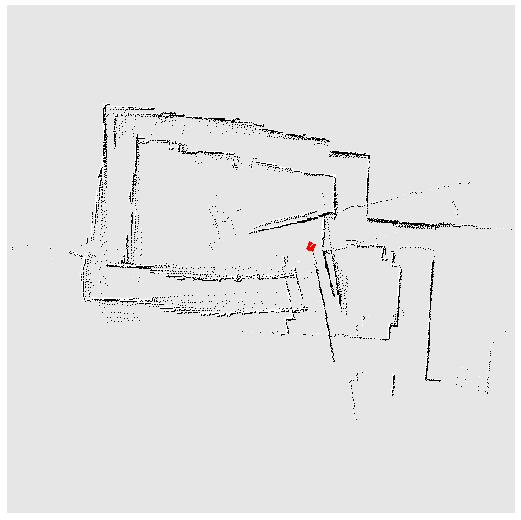
\includegraphics[width=.6\linewidth]{badOdometryMap}
  \caption{Noisy odometry affects map quality}
\end{subfigure}
\begin{subfigure}{.5\textwidth}
  \centering
  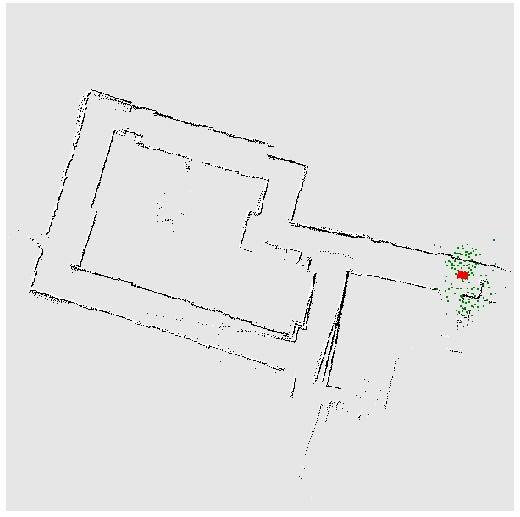
\includegraphics[width=.6\linewidth]{correctedOdometryMap}
  \caption{Corrected map}
\end{subfigure}
\caption[Odometry Errors and Corrected Map]{Use of belief filtering and feature correspondence with loop closure \cite{Thrun}.}
\end{figure}

In order to fix this odometry problem, it is often possible for mobile robots to use trackable shapes in their environment as navigation beacons. Assuming that the walls, doorways, and other measurable objects in the environment are stationary, these can be used as reference points by which to navigate and correct odometry errors. Whereas humans naturally use vision to guide their motion through the world, robots must be explicitly programmed to reconcile the incompatible information coming from odometry, sensors, and any other onboard information sources. Some of the most successful approaches to this reconciliation have relied on probabilistic techniques. By explicitly modeling the noise from various sources of information, it is possible to maintain a probabilistic \textit{belief} about the state of the world and the robot's pose.

With clever implementations, these techniques can be both robust and relatively inexpensive from a computational standpoint. For example, Kalman filtering with Gaussian assumptions about sensor noise creates a loop in which a possible belief about robot state is repeatedly adjusted during actuation and then corrected based on sensor measurements. Due to some convenient mathematical properties of Gaussian distributions, this technique can combine signals to maintain an up to date belief with fairly efficient matrix and arithmetic operations. Even in applications where sensor noise is not exactly Gaussian, techniques like this often work well. Kalman filtering and related methods also rely on sensors and algorithms to perceive the robot's local environment, summarize this perception as a set of key features and their coordinates, and then repeatedly determine which of the features measured at one time correspond to a feature measured afterwards.

%throw some more citations in to this section

While all of these considerations are important for practical robotic mapping operations, they have little to do with the goal of discovering a time efficient multi agent path through an environment with the goal of achieving coverage. In addition, many realistic search and rescue scenarios involving drones may have reasonably accurate compass and GPS signals onboard the drones. While these signals are by no means free of noise, they do not suffer from the cumulative error development that tends to occur when using odometry. In addition, a large amount of robot mapping research applies to mobile robots measuring feature rich indoor settings with sophisticated sensors such as lidar. Because drones are unlikely to carry a lidar or any comparably useful distance measurement sensor, many of the techniques and results from mapping don't apply here. Nonetheless, mapping research is likely to have considerable applicability in a realistic search and rescue scenario. This is particularly true if the environment being explored is largely unknown or significantly changed by a recent disaster. Thus, while the goals and methods of robotic mapping do not apply to this work, it would surely be necessary to combine mapping approaches with the techniques here in order to produce a holistically useful robotic answer to the problems of search and rescue.

\subsection{Applications and Other Notes}

As has been stated throughout this introduction, the following work addresses robotic coverage from a mathematically idealized point of view. However, there are many high quality publications addressing techniques to handle sensor data and noise, actuation and control, localization, and a host of other important concerns. Some examples follow:

CWRU Cutter, a robotic lawn mowing robot developed by the lab of Prof. Roger Quinn at Case Western Reserve University, required lots of effort addressing these practical issues. This includes work by Beno on the mechanical considerations of the project \cite{Beno}, work by Hughes on navigation \cite{Hughes}, and work by Kreinar on localization and odometry noise handling \cite{Kreinar}.

In a 2003 article for the International Journal of Robotics Research, \citeauthor{Acar} develop a robotic mine and unexploded ordinance removal system. Here, the use of a complete coverage algorithm makes sure that all potentially mine filled areas are passed over. The coverage approach used the detection of critical points to perform an exact cellular decomposition of the coverage area. Making this work on a real robot required robotic perception techniques that could go from range sensor data. 